%This is a very basic  BE PROJECT PRELIMINARY template.

%############################################# 
%#########Author :  PROJECT###########
%#########COMPUTER ENGINEERING############


\documentclass[oneside,a4paper,12pt]{report}
%\usepackage{showframe}
%\hoffset = 8.9436619718309859154929577464789pt
%\voffset = 13.028169014084507042253521126761pt

\fancypagestyle{plain}{%
  \fancyhf{}
  \fancyfoot[CE]{College_Name, Department of Computer Engineering 2015}
  \fancyfoot[RE]{\thepage}
}
\pagestyle{fancy}
\fancyhead{}
\renewcommand{\headrulewidth}{0pt}
\footskip = 0.625in
\cfoot{}
\rfoot{}

\usepackage[]{hyperref}
\usepackage{tikz}
\usetikzlibrary{arrows,shapes,snakes,automata,backgrounds,petri}

\usepackage{tabularx}

\usepackage[nottoc,notlot,notlof,numbib]{tocbibind}
\usepackage[titletoc]{appendix}
\usepackage{titletoc}

\renewcommand{\appendixname}{Annexure}
\renewcommand{\bibname}{References}

\setcounter{secnumdepth}{5}

\usepackage{float}
\usepackage{subcaption}
\usepackage{multirow}

\usepackage[ruled,vlined]{algorithm2e}

\begin{document}

\setlength{\parindent}{0mm}
\begin{center}
{\bfseries SAVITRIBAI PHULE PUNE UNIVERSITY \\}
 \vspace*{1\baselineskip}
{\bfseries A PRELIMINARY PROJECT REPORT ON \\}
 \vspace*{2\baselineskip}
{\bfseries \fontsize{16}{12} \selectfont Detection Of Cyber bullying On Social Media Using Machine Learning \\ \vspace*{2\baselineskip}}
{\fontsize{12}{12} \selectfont SUBMITTED TOWARDS THE
 \\PARTIAL FULFILLMENT OF THE REQUIREMENTS OF \\

\vspace*{2\baselineskip}}
{\bfseries \fontsize{14}{12} \selectfont BACHELOR OF ENGINEERING (Computer
Engineering) \\
\vspace*{1\baselineskip}} 
{\bfseries \fontsize{14}{12} \selectfont BY \\ 
\vspace*{1\baselineskip}} 
Student Name  \hspace{25 mm} Exam No:  \\
Student Name \hspace{25 mm} Exam No:   \\
Student Name \hspace{25 mm} Exam No:  \\
Student Name \hspace{25 mm} Exam No:\\
\vspace*{2\baselineskip}
{\bfseries \fontsize{14}{12} \selectfont Under The Guidance of \\  
\vspace*{2\baselineskip}} 
Prof. Guide Name\\
\includegraphics[width=100pt]{collegelogo.png} \\
{\bfseries \fontsize{14}{12} \selectfont DEPARTMENT OF COMPUTER ENGINEERING \\
College Name \\
College Address 
}
\end{center}

\newpage



\begin{figure}[ht]
\centering
\includegraphics[width=100pt]{collegelogo.png}
\end{figure}


{\bfseries \fontsize{14}{12} \selectfont \centerline{College Name}
\centerline{DEPARTMENT OF COMPUTER ENGINEERING}
\vspace*{3\baselineskip}} 


{\bfseries \fontsize{16}{12} \selectfont \centerline{CERTIFICATE} 
\vspace*{3\baselineskip}} 

\centerline{This is to certify that the Project Entitled}
\vspace*{1\baselineskip} 


{\bfseries \fontsize{14}{12} \selectfont \centerline{Detection Of Cyber bullying On Social Media Using Machine Learning}
\vspace*{1\baselineskip}}

\centerline{Submitted by}
\vspace*{1\baselineskip} 
\centerline{Student Name  \hspace{25 mm} Exam No: } 
\centerline{Student Name \hspace{25 mm} Exam No:  } 
\centerline{Student Name \hspace{25 mm} Exam No: }
\centerline{Student Name \hspace{25 mm} Exam No: }
\vspace*{1\baselineskip} 
is a bonafide work carried out by Students under the supervision of Prof. Guide Name and it
is submitted towards the partial fulfillment of the requirement of Bachelor of Engineering (Computer Engineering) Project.\\\\\\

\bgroup
\def\arraystretch{0.7}
\begin{tabular}{c c }
Prof. Guide Name &  \hspace{50 mm} Prof. HOD Name \\								
Internal Guide   &  \hspace{50 mm} H.O.D \\
Dept. of Computer Engg.  &	\hspace{50 mm}Dept. of Computer Engg.  \\
\end{tabular}
%}



\newpage

%\pictcertificate{TITLE OF BE PROJECT}{Student Name}{Exam Seat No}{Guide Name}
\setcounter{page}{0}
\frontmatter
\cfoot{College Short Form Name, Department of Computer Engineering 2021}
\rfoot{\thepage}
\pagenumbering{Roman}
%\pictack{BE PROJECT TITLE}{Guide Name}

		
{  \newpage {\bfseries \fontsize{14}{12} \selectfont \centerline{Abstract} 
In the modern era, the usage of internet has increased
tremendously which in turn has led to the evolution of large
amount of data .Cyber world has its own pros and cons. One of
the alarming situations in web 4.0 is cyber bullying a type of
cyber-crime. When the bullying occurs on line with the aid of
technology it is known as cyber bullying. This research paper
have surveyed the work done by 30 different researchers on
cyber bullying, and elaborated on different methodologies
adopted by them for the detection of bullying.
Cyber-crimes involve all the crimes where internet
is used as an access medium and committed through some
electronic device such as computers and mobile phones.
Unavailability of datasets, hidden identity of predators and the
privacy of the victims are the main factors for limiting the past
research in cyberbullying detection. Considering these factors, an
effective text mining approach using machine learning
algorithms is proposed to proactively detect bullying text. The
dataset collected from myspace.com and Preverted-Justice.com
has been used to evaluate the system’s performance. Three types
of feature namely textual, behavioral and demographic features
are extracted from the dataset as compared to earlier study over
the same dataset where only textual features were considered.
Textual features include certain bullying words that if exists
within the text may lead to a true outcome for cyberbullying.
Personality trait features are extracted for the user if it is
involving once in bullying may bully in future too. While
demographic features extracted from dataset include age, gender
and location. The system is evaluated through different
performance measures for both classifiers used and the
performance of Support Vector Machine classifier is found better
than the Bernoulli NB with an overall 87.14% of classification
accuracy.%, which is suitable for computer aided diagnosis (CAD) of malaria according to world health organization (WHO) quality control standards.\\
\vspace*{2\baselineskip}} \setlength{\parindent}{11mm} }
{ \setlength{\parindent}{0mm} }


{  \newpage {\bfseries \fontsize{14}{12} \selectfont \centerline{Acknowledgments} 
\vspace*{2\baselineskip}} \setlength{\parindent}{11mm} }
{ \setlength{\parindent}{0mm} }
Please Write here Acknowledgment.Example given as\\
\textit{It gives us great pleasure in presenting the preliminary project report 
on {\bfseries \fontsize{12}{12} \selectfont `Detection Of Cyber bullying On Social Media Using Machine Learning'}.}
\vspace*{1.5\baselineskip}

 \textit{I would like to take this opportunity to thank my internal guide
 \textbf{Prof. Guide Name} for giving me all the help and guidance I needed. I am
 really grateful to them for their kind support. Their valuable suggestions were very helpful.} \vspace*{1.5\baselineskip}

 \textit{I am also grateful to \textbf{Prof. HOD Name}, Head of Computer
 Engineering Department, CollegeName for his indispensable
 support, suggestions.}
\vspace*{1.5\baselineskip}

\textit{In the end our special thanks to \textbf{Other Person Name} for
providing various resources such as  laboratory with all needed software platforms,
continuous Internet connection, for Our Project.}
\vspace*{3\baselineskip} \\
\begin{tabular}{p{8.2cm}c}
&Student Name1\\
&Student Name2\\
&Student Name3\\
&Student Name4\\
&(B.E. Computer Engg.)
%}
\end{tabular}


% \maketitle
\tableofcontents
\listoffigures 
%\listoftables



\mainmatter


  \titleformat{\chapter}[display]
{\fontsize{16}{15}\filcenter}
{\vspace*{\fill}
 \bfseries\LARGE\MakeUppercase{\chaptertitlename}~\thechapter}
{1pc}
{\bfseries\LARGE\MakeUppercase}
[\thispagestyle{empty}\vspace*{\fill}\newpage]







\setlength{\parindent}{11mm}
\chapter{Introduction}
\section {Overview}
\item Across the globe due to the tremendous increase in the
availability of data services, addiction of social media among
the society has increased proportionally. Just like other
countries, India has also witnessed a drastic rise in the cyber
bullying. In this era of web 4.0 where people live in digital
and online platforms, it is very difficult to protect the society
from the alarming rise in cyber-crime. It has been surveyed
that the major victims of cyber bullying are adolescents.
Different cyber bullying attacks that are performed by
attacker are: (1) Sending or posting hateful or abusive
comments with an intention to harm the character of an
individual (2) Posting an inappropriate image or video. (3)
Creation of a false or improper website.(4) Issuing online
threats that cause a person to kill themselves or injure another
person. (5) Triggering online religious, racial, ethnic or
political hatred by posting hate comments or videos.
 \\

\subsection{Motivation}
\label{sec:problem}
\item The main Motivation is to Avoid Cyber Bullying and save student or any human life.
Although some users indicate they are being sarcastic, most of them do not. Therefore, it might be indispensable to and a way to automatically detect any sarcastic messages 
Cyber bullying is threatening and destructive act which may result in suicide attempts or negative impact can cause life-long harms to the victims.
The detection of Cyber bullying can be considered as a classification problem. An online post can be classified as a bullying post or normal post.
We will develop a system by applying different machine learning methods to better detect Cyber bullying and improve performance. For example, the Support Vector Machine(SVM), Forest Classifier \\

\subsection{Objective}
\label{sec:problem}
\begin{itemize}


\item   to  The objective of the system is to reveal, analyze and stop cyber bullying in social    media applications. 
 To identify the occurrence of cyber bullying activity in social media platform which helps the government to yield force before many end-users enhance their Target of cyber bullying.
To The system is to give alert message like to warn them, and to identify short hand text and human aggressive behavior on the comment sections. 
To  Also to generate a report which contains the details of bully, and to keep track of count and also by blocking that person along his comment without letting it reach to victim.
\end{itemize}


\chapter{Literature Survey}
\section {Study Of Research Paper}
\item \textbf{1.Paper Name:} Rapid Cyber-bullying detection method using
Compact BERT Models
\\
\textbf{Author:}Mitra Behzadi, Ian G. Harris, Ali Derakhshan  \\
\textbf{Abstract :}:- Nowadays, many people use their social media
platform to spread hate online and that is why the problem of
cyber-bullying detection has been the focus of many researchers
over the past decade. In this work, we tackle this problem
with transfer learning. We use various compact BERT models
and fine-tune them with hate-speech data. We incorporate Focal
Loss function to handle class imbalance in the data. Using this
approach, we were able to achieve state-of-the-art results of 0.91
precision, 0.92 recall and 0.91 F1-score on the hate-speech dataset.
Additionally, using our transfer learning pipeline, we show
that the more compact BERT models are significantly faster in
detection and are suitable for real-time applications of cyberbullying
detection.  \\

\newpage

\item \textbf{ 2.Paper Name:} :- Review of Machine Learning methods
for Identification of Cyberbullying in
Social Media\\
\textbf{Author:}Neha Singh, Sanjay Kumar Sharma\\
\textbf{Abstract :} In the modern era, the usage of internet has increased
tremendously which in turn has led to the evolution of large
amount of data .Cyber world has its own pros and cons. One of
the alarming situations in web 4.0 is cyber bullying a type of
cyber-crime. When the bullying occurs on line with the aid of
technology it is known as cyber bullying. This research paper
have surveyed the work done by 30 different researchers on
cyber bullying, and elaborated on different methodologies
adopted by them for the detection of bullying, and how you
protect the society from online evil act of cyber bullying.  \\ 
	
\newpage
	
\item \textbf{3.Paper Name:}A Fairness-Aware Fusion Framework for Multimodal Cyberbullying Detection  \\
\textbf{Author:}Jamal Alasadi,Ramanathan Arunachalam ,Pradeep K. Atrey, Vivek K. Singh \\
\textbf{abstract :} Recent reports of bias in multimedia algorithms
(e.g., lesser accuracy of face detection for women and persons of
color) have underscored the urgent need to devise approaches
which work equally well for different demographic groups.
Hence, we posit that ensuring fairness in multimodal cyberbullying
detectors (e.g., equal performance irrespective of the
gender of the victim) is an important research challenge. We
propose a fairness-aware fusion framework that ensures that
both fairness and accuracy remain important considerations
when combining data coming from multiple modalities. In
this Bayesian fusion framework, the inputs coming from
different modalities are combined in a way that is cognizant
of the different confidence levels associated with each feature
and the interdependencies between features. Specifically, this
framework assigns weights to different modalities not just
based on accuracy but also their fairness. Results of applying
the framework on a multimodal (visual + text) cyberbullying
detection problem demonstrate the value of the proposed
framework in ensuring both accuracy and fairness. % accuracy for detection and counting of RBCs and 100% for detection and classifying the parasite into one of its four types. \\
\newpage

\item \textbf{4.Paper Name:}Text Imbalance Handling and Classification for Cross- platform Cyber-crime Detection using Deep Learning\\
\textbf{Author:}:-Munipalle Sai Nikhila, Aman Bhalla , Pradeep Singh \\
\textbf{abstract :}Cyberbullying has become a very prevalent issue in recent times. Not just qualifying this as a women issue, starting from politicians to a ten-year-old kid, every person is being bullied on any social platform. It is highly essential to build an artificial intelligence based model that detects the presence of bullying in cross-platform posts. However, textual datasets which are useful for model generation are highly imbalanced in nature. In this paper, we propose two main methods to handle textual data imbalancing which are synonym replacement and artificial data generation using generative adversarial neural networks. We present a systematic analysis of our approaches using a convolutional neural network classifier. Our work shows how removing data imbalance with generative adversarial network techniques before classification improves the overall performance of the model.% and sensitivity of 95.2% for malaria parasite detection, and an accuracy of 87.9% for identifying the two species Plasmodium falciparum and Plasmodium vivax.\\

\newpage

\item \textbf{5.Paper Name:}Cyber Bullying and the Expected Consequences on the Students’ Academic Achievement\\
\textbf{Author:}Norah Basheer Alotaibi\\
\textbf{Abstract:}In the Saudi school system, cyber bullying is a persistent problem perpetuated by the development of digital technology and its ubiquitous presence in almost every societal aspect. With such technologies, it is not surprising that harassment has proliferated to the virtual world of teenagers, within which harassment is rampant. This phenomenon’s frequency and outcomes have alarmed stakeholders but surprisingly, studies examining the causes and motivations behind cyber space bullying engagement are few and far between. This issue was examined through the lens of a well-known theory, the Theory of Planned Behavior (TPB). More specifically, this study examined the effects of attitudes, normative beliefs, subjective norms, and perceived behavioral control/self-efficacy on intentions towards cyber bullying and expected societal outcomes. The study distributed 395 questionnaires to high school students in the 9th to 12th grades in Saudi schools. The gathered data was run through multiple linear regressions, after which the findings showed that behavioral attitudes, social norms, perceived behavioral controls, social media use, a lack of parental controls, and a lack of regulations had a direct effects on intentions towards cyber bullying. The findings also indicated that intentions towards cyber bullying had a direct effect on student academic performance. This study provides valuable information concerning intentions towards cyberspace bullying among students and the relationship between Theory of Planned Behavior (TPB) variables and the predictive utility model. Finally, this study’s findings are a basis upon which prevention and intervention strategies can be developed, which has many implications for theory, practice, and policy.  \\

\newpage

\item \textbf{6.paper Name:}Identification and Classification of Cybercrimes using
Text Mining Technique\\
\textbf{Author:}Shiza Andleeb,Dr. Rashid Ahmed, Zaheer Ahmed, Maira Kanwal\\
\textbf{Abstract:}Cyber-crimes involve all the crimes where internet
is used as an access medium and committed through some
electronic device such as computers and mobile phones.
Unavailability of datasets, hidden identity of predators and the
privacy of the victims are the main factors for limiting the past
research in cyberbullying detection. Considering these factors, an
effective text mining approach using machine learning
algorithms is proposed to proactively detect bullying text. The
dataset collected from myspace.com and Preverted-Justice.com
has been used to evaluate the system’s performance. Three types
of feature namely textual, behavioral and demographic features
are extracted from the dataset as compared to earlier study over
the same dataset where only textual features were considered.
Textual features include certain bullying words that if exists
within the text may lead to a true outcome for cyberbullying.
Personality trait features are extracted for the user if it is
involving once in bullying may bully in future too. While
demographic features extracted from dataset include age, gender
and location. The system is evaluated through different
performance measures for both classifiers used and the
performance of Support Vector Machine classifier is found better
than the Bernoulli NB with an overall 87.14% of classification
accuracy.\\

\newpage
\item \textbf{7. Paper Name:}A Bag-of-Phonetic-Codes Model for Cyber-Bullying Detection in Twitter\\
\textbf{Author:}Ankita Shekhar ,M. Venkatesan\\
\textbf{Abstract:}Social networking sites such as Twitter, Facebook, MySpace, Instagram are emerging as a strong medium of communication these days. These have become a part and parcel of daily life. People can express their thoughts and activities among their social circle with brings them closer to their community. However this freedom of expression has its drawbacks. Sometimes people show their aggression on Social Media which in turn hurts the sentiments of the targeted victims. Certain forms of cyber-bullying are sexual, racial and physical disability based. Hence a proper surveillance is necessary to tackle such situations. Twitter as a micro-blogging site sees cyber abuse on a daily basis. However, tweets are raw texts; containing a lot of misspelled words and censored words. This paper proposes a novel method to detect cyber-bullying, a Bag-of-Phonetic-Codes model. Using pronunciation of words as features can rectify misspelled words and can identify censored words. Correctly identifying duplicate words can lead to smaller vocabulary of words, thereby reducing the feature space. The inspiration for this proposed work is drawn from the famous Bag-of-Words model for extracting textual features. Phonetic code generation has been done using the Soundex Algorithm. Besides the proposed model, experiments were carried out with both supervised and unsupervised machine learning approaches on multiple datasets to understand the approaches and challenges in the domain of cyber-bullying detection. %80, %83, %86, %75 precision
%, 86%, 86%, 79% f-measure on 19 test images.\\
\newpage
\item \textbf{8.Paper Name:}Cyber-Smart Children, Cyber-Safe Teenagers:
Enhancing internet Safety for Children\\
\textbf{Author:}Tracy WERU1, Joseph SEVILLA2 , John OLUKURU3,
Lorna MUTEGI4,Tabitha MBERI5\\
\textbf{Abstract:}- Millennials have access to online resources vastly beyond what their
parents had, and beyond what some teachers even understand. In most cases,
children are more technologically advanced than adults, so(therefore) adults feel
intimidated and refrain from enforcing rules that are imperative to protect their
children as they access resources online. Amidst the increase in cybercrimes
globally, Kenyan children are becoming potential targets on the internet as the
country struggles with a feeble Children’s Act 2001 which fails to provide sufficient
protection to victims as well as stringent penalties to the offenders. The Children’s
Act 2001 which safeguards the child from both physical and psychological abuse,
does not provide sufficient provisions to protect the child from cybercrimes such as
cyber bullying, pornography, lottery scams, pseudo-attacks among others. This paper
illustrates the importance of a mobile game application designed specifically for
children, teachers and parents to educate them on Cyber safety\\
\newpage
\item \textbf{9.Paper name:}Identification of Potential Cyber Bullying Tweets
using Hybrid Approach in Sentiment Analysis\\
\textbf{Author:} Akankshi Mody , Shreni Shah , Reeya Pimple ,Narendra Shekokar\\
\textbf{Abstract:}—With the rise of the Internet, cyber bullying is
becoming more and more widespread. Cyber bullying has
resulted in such disastrous consequences that there is a pressing
need to detect it. The aim of this study is to do the same by using
sentiment analysis. We perform cyber bullying detection using a
novice approach on Tweets using Natural Language Processing
and Machine Learning techniques. After processing a tweet, it
can be flagged down if the tweet is a potential cyber bullying
threat.\\
\newpage

\item \textbf{10. Paper Name:}Analysis of Cyber Aggression and Cyber-bullying in Social Networking \\
\textbf{Author:}Tadashi Nakano1, Tatsuya Suda2, Yutaka Okaie1, and Michael John Moore3\\
\textbf{Abstract:}This paper considers Ask.fm, a social networking
site where users create profiles and can send each other
questions, and analyses aggressive user behavior that may
potentially lead to cyber-bullying incidents. We hypothesize
that anonymity is a primary cause of such aggressive user
behavior and examine how anonymous and non-anonymous
users behave in social networking. We collected data from
Ask.fm and analyzed questions posted by anonymous and
non-anonymous users and answers posted by non-anonymous
users. Analysis of the collected data shows that anonymous
users exhibit more aggressive behavior than non-anonymous
users. Analysis also shows that users become more aggressive
in answering aggressive anonymous questions than aggressive
non-anonymous questions.\\
\chapter{Problem Statement}
\section {Problem Statement}
Cyber bullying is the problem in current Situation of the world Because All  the Student or humans use social media.
we try to avoid Cyber bullying through our project .
The propose is to find an  efficient way to detect sarcastic tweets, and study how to use this information (i.e., whether the tweet is sarcastic or not) to enhance the accuracy of Cyber bullying . 


\chapter{Project Requirement}



\section {EXTERNAL INTERFACE REQUIREMENT}
\subsection {User Interface}
 \item Application Based cyber bullying Detection. 
 
 \subsection {Hardware Interfaces:}
 \item RAM : 8 GB\\
As we are using Machine Learning Algorithm and Various High Level Libraries Laptop\\
RAM minimum required is 8 GB.\\
Hard Disk : 40 GB\\
Data Set of CT Scan images is to be used hence minimum 40 GB Hard Disk memory is required.\\
Processor : Intel i5 Processor\\
Pycharm IDE that Integrated Development Environment is to be used and data loading should be fast hence Fast Processor is required\\
IDE : Pycharm\\
Best Integrated Development Environment as it gives possible suggestions at the time of typing code snippets that makes typing feasible and fast.\\
Coding Language : Python Version 3.5\\
Highly specified Programming Language for Machine Learning because of availability of High Performance Libraries.\\
Operating System : Windows 10\\
Latest Operating System that supports all type of installation and development Environment\\

 \subsection {Software Interfaces}
\item  Operating System: Windows 10\\
\item IDE: Spyder\\
\item Programming Language : Python\\

\section {NON FUNCTIONAL REQUIREMENT}
\subsection {PerformanceRequirements}
\item The performance of the functions and every module must be well. The overallperformance of the software will enable the users to work eciently.  Perfor-mance  of  encryption  of  data  should  be  fast.   Performance  of  the  providingvirtual environment should be fastSafety Requirement•The application is designed in modules where errors can be detected and xedeasily. This makes it easier to install and update new functionality if required.\\
 \subsection {Safety Requirement}
 \item The application is designed in modules where errors can be detected and fixed easily. This makes it easier to install and update new functionality if required.\\
 
\subsection {Software Quality Attributes}
\item  Our software has many quality attribute that are given below:-\\
\item Adaptability: This software is adaptable by all users.\\
\item Availability: This software is freely available to all users. The availability of the software is easy for everyone.\\
\item Maintainability: After the deployment of the project if any error occurs then it can be easily maintained by the software developer.\\
\item Reliability: The performance of the software is better which will increase the reliabilityof the Software.\\
\item User Friendliness: Since, the software is a GUI application; the output generated is much user friendly in its behavior.\\
\item Integrity: Integrity refers to the extent to which access to software or data by unauthorized persons can be controlled.\\
\item Security: Users are authenticated using many security phases so reliable security is provided.\\
\item Testability: The software will be tested considering all the aspects.\\
\newpage
\chapter {System Analysis}
\section {system Architecture}

\begin{figure}[h]
	\centering
		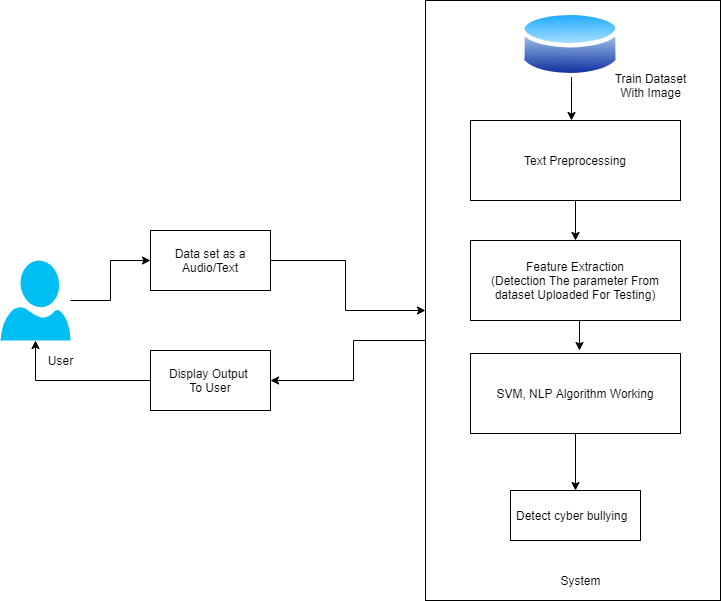
\includegraphics[width=0.90\textwidth]{system architecture.png}
	\caption {system Architecturel}
	\end{figure}\\

\subsection{Module}   
\begin{itemize}
 
\item {Admin}
\item In this module,the Admin has to log in by using valid user name and password. After login successful he can do some operations such as View All Users and Authorize, View All E-Commerce Website and Authorize,View All Products and Reviews,View All Products Early Reviews, View All Keyword Search Details, View All Products Search Ratio, View All Keyword Search Results, View All Product Review Rank Results.\\

\item {View and Authorize Users}
\item In this module, the admin can view the list of users who all registered. In this, the admin can view the user’s details such as, user name, email, address and admin authorizes the users.\\

\item {View Charts Results}
\item View All Products Search Ratio,View All Keyword Search Results,View All Product Review Rank Results.\\

\item {Ecommerce User}
\item In this module, there are n numbers of users are present. User should register before doing any operations. Once user registers, their details will be stored to the database. After registration successful,he has to login by using authorized user name and password Once Login is successful user will do some operations like Add Products, View All Products with reviews, View All Early Product’s reviews, View All Purchased Transactions.\\
\item {End User}
\item In this module, there are n numbers of users are present. User should register before doing any operations. Once user registers, their details will best or to the database. After registration successful,he has to login by using authorized user name and password. Once Login is successful user will do some operations like Manage Account, Search Products by keyword and Purchase, View Your Search Transactions, View.\\
 
\end{itemize}
\subsection {Data Flow Diagram}
%\subsection{Data Flow Diagram}  
\item In Data Flow Diagram,we Show that flow of data in our system in DFD0 we show that base DFD in which rectangle present input as well as output and circle show our system,In DFD1 we show actual input and actual output of system input of our system is text or image and output is rumor detected like wise in DFD 2 we present operation of user as well as admin.\\
\begin{center}
	\begin{figure}[!htbp]
		\centering
		\fbox{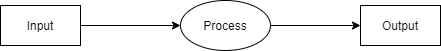
\includegraphics[height=50pt]{dfd0.png}}
	  \caption{Data Flow(0) diagram}
	  \label{fig:act-dig}
	\end{figure}
\end{center}  
\newpage 
\begin{center}
	\begin{figure}[!htbp]
		\centering
		\fbox{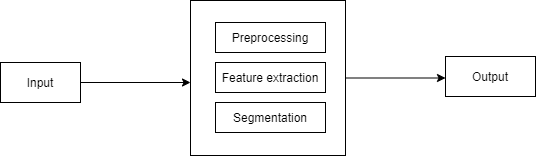
\includegraphics[height=100pt]{dfd1.png}}
	  \caption{Data Flow(1) diagram}
	  \label{fig:act-dig}
	\end{figure}
\end{center}  

\begin{center}
	\begin{figure}[!htbp]
		\centering
		\fbox{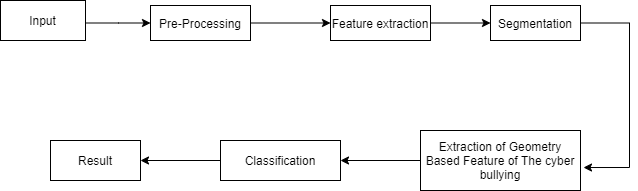
\includegraphics[height=150pt]{dfd2.png}}
	  \caption{Data Flow(2) diagram}
	  \label{fig:act-dig}
	\end{figure}
\end{center}  
\newpage

\section{UML DIAGRAMS} 
\item Unified Modeling Language is a standard language for writing software blueprints.The UML may be used to visualize,specify,construct and document the artifacts of a softwareintensive system.UML is process independent,although optimally it should be used in process that is use case driven,architecture-centric,iterative,and incremental.The Number of UML Diagram is available.\\

 \item Class Diagram.\\
\item Use case Diagram.\\
 \item Activity Diagram.\\
\item Sequence Diagram.\\


 \begin{center}
	\begin{figure}[!htbp]
		\centering
		\fbox{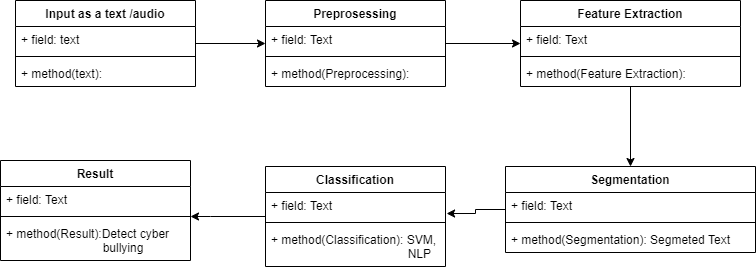
\includegraphics[width=390pt]{class.png}}
	  \caption{Class Diagram Diagram}
	  \label{fig:class-dig}
	\end{figure}
\end{center} 
\newpage
%\subsection{Use Case Diagram}

\begin{center}
	\begin{figure}[!htbp]
		\centering
		\fbox{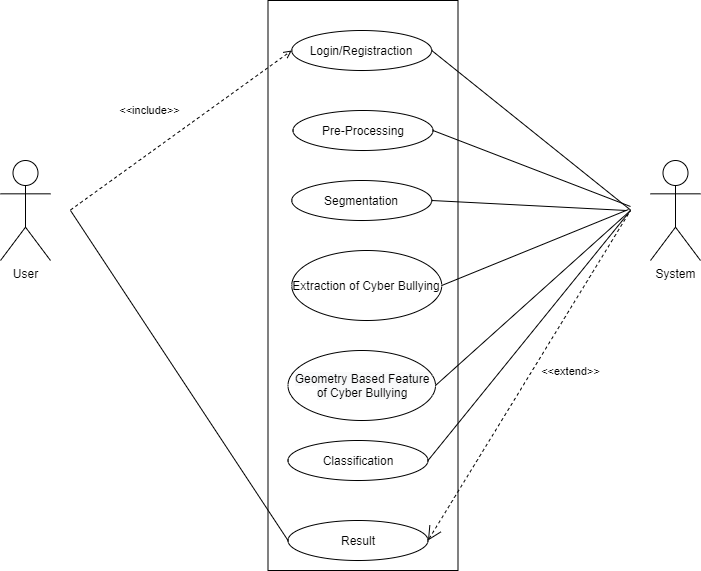
\includegraphics[width=400pt]{use case.png}}
	  \caption{Use case Diagram}
	  \label{fig:class-dig}
	\end{figure}
\end{center} 

\newpage
%\subsection{Activity Diagram}

\begin{center}
	\begin{figure}[!htbp]
		\centering
		\fbox{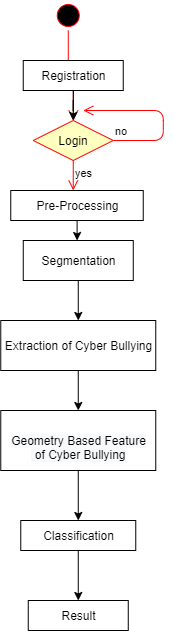
\includegraphics[width=150pt]{Activity.png}}
	  \caption{Activity Diagram}
	  \label{fig:class-dig}
	\end{figure}
\end{center} 
 
\newpage
 
%\subsection{Sequence Diagram}
 \begin{center}
	\begin{figure}[!htbp]
		\centering
		\fbox{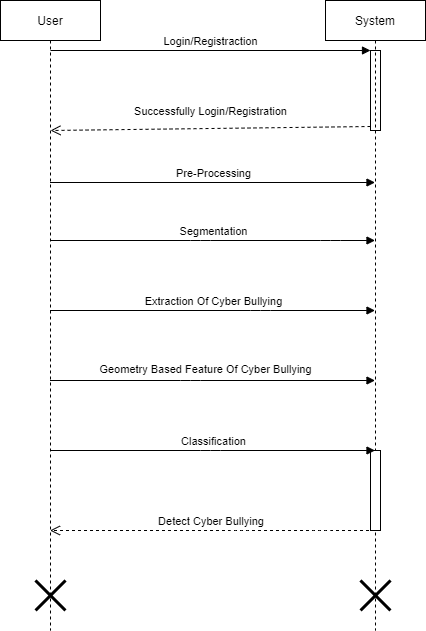
\includegraphics[width=250pt]{Sequence.png}}
	  \caption{Sequence Diagram}
	  \label{fig:class-dig}
	\end{figure}
\end{center}

\chapter{Software Information}

Python is an interpreted, high-level and general-purpose programming language. Created by Guido van Rossum and first released in 1991, Python's design philosophy emphasizes code readability with its notable use of significant whitespace. Its language constructs and object-oriented approach aim to help programmers write clear, logical code for small and large-scale projects.

Python is dynamically typed and garbage-collected. It supports multiple programming paradigms, including structured (particularly, procedural), object-oriented, and functional programming. Python is often described as a "batteries included" language due to its comprehensive standard library.

Python was created in the late 1980s as a successor to the ABC language. Python 2.0, released in 2000, introduced features like list comprehensions and a garbage collection system with reference counting.

Python 3.0, released in 2008, was a major revision of the language that is not completely backward-compatible, and much Python 2 code does not run unmodified on Python 3.

The Python 2 language was officially discontinued in 2020 (first planned for 2015), and "Python 2.7.18 is the last Python 2.7 release and therefore the last Python 2 release."[30] No more security patches or other improvements will be released for it. With Python 2's end-of-life, only Python 3.6.x and later are supported.

Python interpreters are available for many operating systems. A global community of programmers develops and maintains CPython, a free and open-source reference implementation. A non-profit organization, the Python Software Foundation, manages and directs resources for Python and CPython development.\\

Python was conceived in the late 1980s by Guido van Rossum at Centrum Wiskunde & Informatica (CWI) in the Netherlands as a successor to the ABC language (itself inspired by SETL), capable of exception handling and interfacing with the Amoeba operating system. Its implementation began in December 1989. Van Rossum shouldered sole responsibility for the project, as the lead developer, until 12 July 2018, when he announced his "permanent vacation" from his responsibilities as Python's Benevolent Dictator For Life, a title the Python community bestowed upon him to reflect his long-term commitment as the project's chief decision-maker. He now shares his leadership as a member of a five-person steering council. In January 2019, active Python core developers elected Brett Cannon, Nick Coghlan, Barry Warsaw, Carol Willing and Van Rossum to a five-member "Steering Council" to lead the project.\\
\newpage
\textbf{Anaconda:}
Anaconda is a free and open-source distribution of the Python and R programming languages for scientific computing (data science, machine learning applications, large-scale data processing, predictive analytics, etc.), that aims to simplify package management and deployment. The distribution includes data-science packages suitable for Windows, Linux, and macOS. It is developed and maintained by Anaconda, Inc., which was founded by Peter Wang and Travis Oliphant in 2012. As an Anaconda, Inc. product, it is also known as Anaconda Distribution or Anaconda Individual Edition, while other products from the company are Anaconda Team Edition and Anaconda Enterprise Edition, both of which are not free.

Package versions in Anaconda are managed by the package management system conda. This package manager was spun out as a separate open-source package as it ended up being useful on its own and for other things than Python. There is also a small, bootstrap version of Anaconda called Miniconda, which includes only conda, Python, the packages they depend on, and a small number of other packages.
Anaconda distribution comes with over 250 packages automatically installed, and over 7,500 additional open-source packages can be installed from PyPI as well as the conda package and virtual environment manager. It also includes a GUI, Anaconda Navigator, as a graphical alternative to the command line interface (CLI).

The big difference between conda and the pip package manager is in how package dependencies are managed, which is a significant challenge for Python data science and the reason conda exists.

When pip installs a package, it automatically installs any dependent Python packages without checking if these conflict with previously installed packages[citation needed]. It will install a package and any of its dependencies regardless of the state of the existing installation[citation needed]. Because of this, a user with a working installation of, for example, Google Tensorflow, can find that it stops working having used pip to install a different package that requires a different version of the dependent numpy library than the one used by Tensorflow. In some cases, the package may appear to work but produce different results in detail.

In contrast, conda analyses the current environment including everything currently installed, and, together with any version limitations specified (e.g. the user may wish to have Tensorflow version 2,0 or higher), works out how to install a compatible set of dependencies, and shows a warning if this cannot be done.

Open source packages can be individually installed from the Anaconda repository, Anaconda Cloud (anaconda.org), or the user's own private repository or mirror, using the conda install command. Anaconda, Inc. compiles and builds the packages available in the Anaconda repository itself, and provides binaries for Windows 32/64 bit, Linux 64 bit and MacOS 64-bit. Anything available on PyPI may be installed into a conda environment using pip, and conda will keep track of what it has installed itself and what pip has installed.

Custom packages can be made using the conda build command, and can be shared with others by uploading them to Anaconda Cloud, PyPI or other repositories.

The default installation of Anaconda2 includes Python 2.7 and Anaconda3 includes Python 3.7. However, it is possible to create new environments that include any version of Python packaged with conda\\

\newpage 
\textbf{Spyder}

Spyder is a free and open source scientific environment written in Python, for Python, and designed by and for scientists, engineers and data analysts. It features a unique combination of the advanced editing, analysis, debugging, and profiling functionality of a comprehensive development tool with the data exploration, interactive execution, deep inspection, and beautiful visualization capabilities of a scientific package. \\
\textbf{Features}\\
\begin{itemize}
    \itemAn editor with syntax highlighting, introspection, code completion
Support for multiple IPython consoles
The ability to explore and edit variables from a GUI
A Help pane able to retrieve and render rich text documentation on functions, classes and methods automatically or on-demand
A debugger linked to IPdb, for step-by-step execution
Static code analysis, powered by Pylint
A run-time Profiler, to benchmark code
Project support, allowing work on multiple development efforts simultaneously
A built-in file explorer, for interacting with the filesystem and managing projects
A "Find in Files" feature, allowing full regular expression search over a specified scope
An online help browser, allowing users to search and view Python and package documentation inside the IDE
A history log, recording every user command entered in each console
An internal console, allowing for introspection and control over Spyder's own operation\\
\end{itemize}

\chapter{Project Plan}

In this chapter we are going to have an overview about how much time does it took to complete each task like- Preliminray Survey Introduction and Problem Statement, Literature
Survey, Project Statement, Software Requirement and Specification, System Design, Partial
Report Submission, Architecture Design, Implementation, Deployment, Testing, Paper Publish, Report Submission and etcetera. This chapter also gives focus on stakeholder list which
gives information about project type, customer of the proposed system, user and project
member who developed the system.\\

\section{Stakeholder List}




\section{System Implementation Plan}

The System Implementation plan table, shows the overall schedule of tasks compilation and
time duration required for each task.

\begin{center}

\begin{tabular}{|c|p{6cm}|p{3cm}|p{3cm}|}
\hline
\textbf{Sr. No.} & \textbf{Name/Title} & \textbf{Start Date}& \textbf{End Date} \\

\hline
1& Preliminary Survey& &  \\
\hline
2& Introduction and Problem Statement
&  &  \\
\hline
3& Literature Survey&      &   \\
\hline
4& Project Statement
&  & \\
\hline
5& Software Requirement And Specification &    & \\
\hline
6 & System Design &  & \\
\hline
7 & Partial Report Submission &  &     \\
\hline
8 & Architecture Design &      &    \\
\hline
9 & Implementation
 &    & \\
\hline
10 & Deployement &      &   \\
\hline
11 & Testing &  &  \\
\hline
12 & Paper Publish
 &  & \\
\hline
13 & Report Submission
 &  &  \\
\hline

\end{tabular}  
%\caption{Schedule of the Project 1}
\end{center}





 \chapter{Conclusion}
 \section {Conclusion}
\item In this work, a system is proposed which detects on English as well as on Hindi tweets in Twitter. Cyber bullying is very dependent and highly contextual; therefore, sentiment and other contextual clues to help detect the Cyber bullying . The system uses sarcastic tweets, 9,104 tweets containing Cyber bullying , and #not dataset. The system uses the LR Algorithm . The approach has shown good results and it is observed that LR classifier has more accuracy than other classifier. All patterns for sarcastic detection are not covered in the extracted patterns. 
From the survey it can be
concluded that the traditional machine learning algorithms
are incapable of handling the enormous amount of data
being generated in Web 4.0 moreover the cyber bullying
content cannot be detected accurately .Recently Deep
learning techniques, NLP, deep recurrent neural
network,CNN, stacked auto-encoder,has gained the
attention of many researchers.Future work can target on
usage of these deep learning techniques for precise detection
of cyberbullying in social media.Lot of research is being
conducted in the field of cyberbullying. It is an emerging
issue which needs to be addressed in Web 4.0 .After
reviewing the 30 research papers it found that there is a lack
of proper dataset, collecting huge dataset is a major
challenge, integrating social, contextual, sentiment features
can improve the accuracy of detection of bullying content.
For future work, data from multiple social media platforms
can be considered , apart from text, image , video must be
taken into account for experimentation.
\\

\bibliographystyle{ieeetr}
\bibliography{biblo}
\begin{itemize}
   
\item [1] Y. Bengio, A. Courville, and P. Vincent, “Representation learning: A review and new perspectives,” Pattern Analysis and Machine Intelligence, IEEE Transactions on, vol. 35, no. 8, pp. 1798–1828, 2013 \\

\item [2]A. M. Kaplan and M. Heinlein, “Users of the world, unite! The challenges and opportunities of social media,” Business horizons, vol. 53, no. 1, pp. 59–68, 2010. \\

\item [3] ] R. M. Kowalski, G. W. Giumetti, A. N. Schroeder, and M. R.Lattanner, “Bullying in the digital age: A critical review and misanalysis of cyber bullying research among youth.” 2014\\

\item [4]B. K. Biggs, J. M. Nelson, and M. L. Sampilo, “Peer relations in the anxiety–depression link: Test of a mediation model,” Anxiety, Stress, & Coping, vol. 23, no. 4, pp. 431–447, 2010. \\

\item [5] K. Dinakar, B. Jones, C.Havasi, H. Lieberman, and R. Picard. "Common
sense reasoning for detect ion, prevent ion, and mit igat ion of
cyberbullying." ACM Transact ions on Interactive Intelligent Systems
(TiiS) 2, no. 3, 2012, p. 18. \\


\item [6]V. Nahar, S. Unankard, X. Li, and C. Pang. "Sent iment analysis for
effective detect ion of cyber bullying." In Asia-Pacific Web Conference,
Springer, Berlin, Heidelberg, 2012, pp. 767-774.\\

\item [7] V. Nahar, X. Li, C. Pang, and Y. Zhang. "Cyberbullying detect ion based
on text-st ream classification." In The 11th Aust ralasian Data Mining
Conference (AusDM 2013), 2013.\\

\item [8] ] M. Dadvar, D. Trieschnigg, R. Ordelman, and F. de Jong. "Improving
cyberbullying detect ion with user context ." In European Conference on
Information Retrieval, Springer, Berlin, Heidelberg, 2013, pp. 693-696.\\

\item [9]] V. Nahar, S. Al-Maskari, X. Li, and C. Pang. "Semi-supervised learning
for cyberbullying detect ion in social networks." In Aust ralasian
Database Conference, Springer, Cham, 2014, pp. 160- 171.\\

\item [10]V. Nahar, X. Li, H. L. Zhang, and C. Pang. "Detecting cyberbullying in
social networks using mult i-agent system." Web Intelligence and Agent
Systems: An International Journal 12, no. 4, 2014, pp. 375- 388\\





\end{itemize}
\begin{appendices}

\end{appendices}
\end{document}
